\documentclass[]{IEEEtran}

\usepackage[italian]{babel}
\usepackage{microtype}
\usepackage{graphicx}
\usepackage{float}
\usepackage[export]{adjustbox}
\usepackage{dirtree}
\usepackage{hyperref}
\usepackage{tikz}
\usepackage{url}
\usepackage[scale=0.94]{inconsolata}

% tabella dei risultati
\usepackage{array}
\usepackage{siunitx}
\usepackage{booktabs}

\newcommand{\ScanTrans}{\textrm{ScanTrans}}
\newcommand{\MergeTrans}{\textrm{MergeTrans}}
\newcommand{\BlockSize}{\textrm{BLOCK\_SIZE}}
\newcommand{\SplitterDistance}{\textrm{SP\_DIST}}
\newcommand{\cuSPARSE}{\textrm{cuSPARSE}}
\newcommand{\var}[1]{\texttt{#1}}

\graphicspath{{figures/}} 	

\title{Sparse Matrix Transposition for GPUs}
\author{\begin{tabular}{c c}
    Massimiliano Incudini & VR433300\\
    Michele Penzo & VR439232
\end{tabular}}

\begin{document}
\maketitle

\begin{abstract}
Il progetto implementa diversi algoritmi paralleli per calcola la \emph{trasposta} di una matrice \emph{sparsa}, estendendo \cite{parallelTrans} riscrivendo il software per GPU NVidia attraverso il linguaggio CUDA. 
I risultati ottenuti vengono confrontati con le tempistiche della stessa operazione esposta dalla libreria \cuSPARSE, parte dell'SDK di NVidia. Infine suggeriamo alcune modifiche per migliorare ulterioremente le performance degli algoritmi da noi implementati.

\end{abstract}

\begin{figure*}[t]
    \centering
	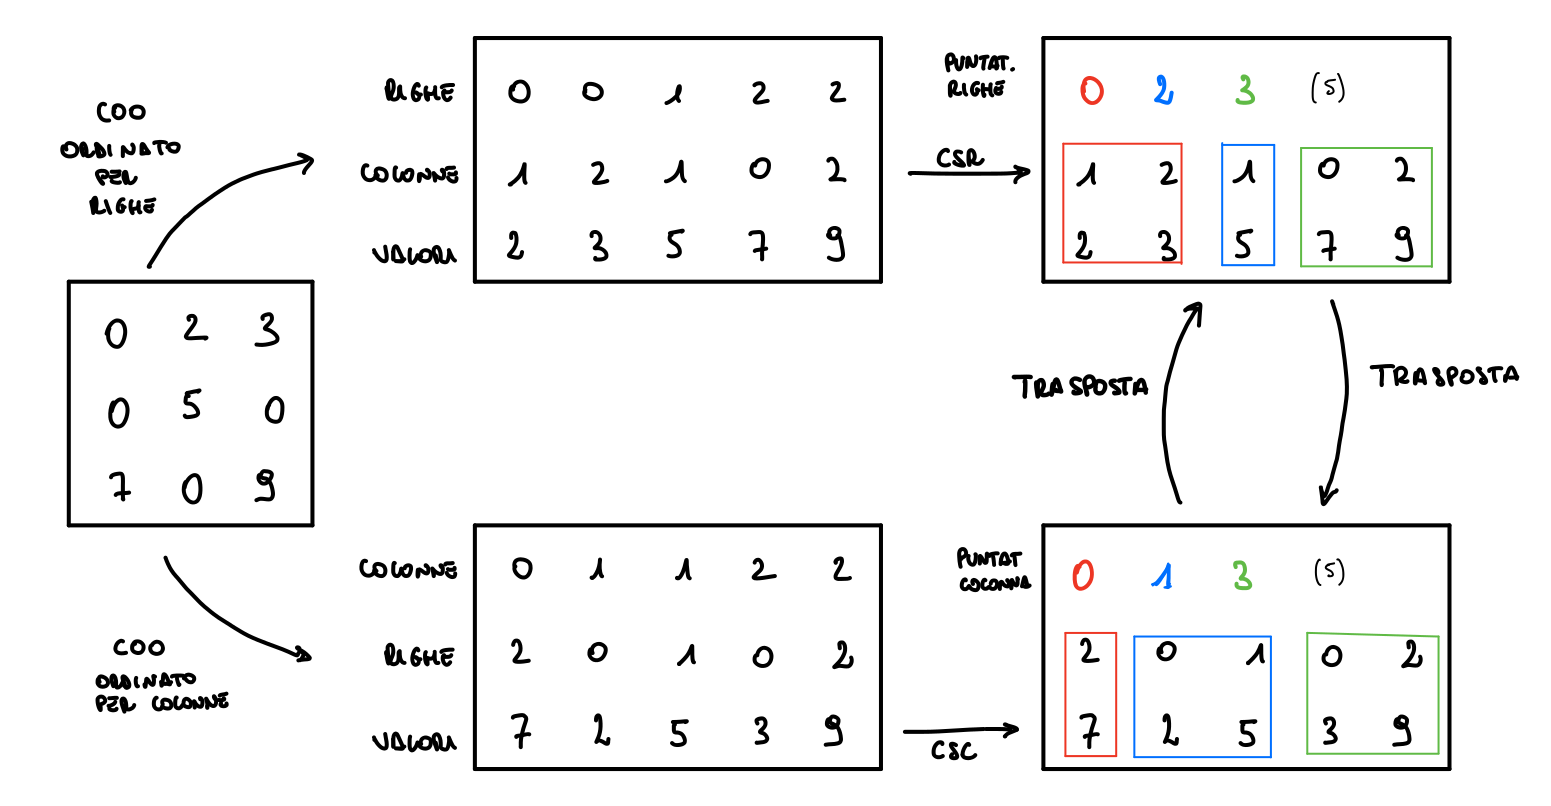
\includegraphics[scale=0.25]{conceptual_transpose.png}
	\caption{Trasformazione da formato esteso a CSR, oppure CSC}
	\label{first_fig}
\end{figure*}


\section{Introduzione e motivazioni}\label{introduzione}

Diverse applicazioni in ambito scientifico utilizzano le matrice sparse per rappresentare in modo compatto ed efficiente matrici e grafi. 

La operazioni fondamentali per poter lavorare su tali strutture sono la moltiplicazione e la \emph{trasposta}. In questo lavoro abbiamo ci siamo concentrati su questa seconda operazione. La trasposta è una componente fondamentale di diversi algoritmi come descritto in \cite{parallelTrans}.

Verranno quindi mostrate le basi per la rappresentazione, i problemi riscontrati durante lo sviluppo e analizzati alcuni algoritmi per il calcolo su GPU.

\section{Rappresentazione delle matrici}\label{rappresentazione}

Una matrice viene definita sparsa quando la maggior parte dei suoi valori sono nulli. Non esiste una definizione precisa, se consideriamo però una matrice di dimensioni $m \times n$ possiamo definire sparsa una matrice il cui numero di elementi non nulli $\mathrm{nnz}$ è più vicina ad $\max\{m, n \}$ che ad $m \times n$. 

Tutti i formati di matrice sparsa permettono di memorizzare la matrice in modi molto più efficiente dal punto di vista dello storage. Alcuni formati permettono una più veloce modifica (es: \emph{formati COO}) altri invece un più efficiente accesso al dato (es. \emph{formati CSR, CSC}). 

Una panoramica dei formati è presente in Figura~\ref{first_fig}.

\subsection{Formato COO}

Il formato COO (\emph{COOrdinate}) rappresenta la matrice di dimensioni $m \times n$ ed $\mathrm{nnz}$ elementi non nulli attraverso tre vettori di lunghezza $\mathrm{nnz}$:
\begin{itemize}
    \item \var{coo\_val}: contiene i valori non nulli;
    \item \var{coo\_row\_idx}: contiene gli indici di riga dei valori non nulli;
    \item \var{coo\_col\_idx}: contiene gli indici di colonna dei valori non nulli.
\end{itemize}

Per un accesso efficiente al dato occorre mantenere i vettori ordinati \emph{per indice di riga} oppure per \emph{indice di colonna}. 

\subsection{Formato CSR}\label{csr}

Il formato CSR (\emph{Compressed Sparse Row}) rappresenta la matrice di dimensioni $m \times n$ ed $\mathrm{nnz}$ elementi non nulli attraverso un vettore di lunghezza $m+1$ e due vettori di lunghezza $\mathrm{nnz}$. Può essere efficientemente ottenuto partendo dal formato \emph{COO ordinato per righe}. 
\begin{enumerate}
\item \var{csr\_row\_ptr}: ottenuto processando il vettore \var{coo\_row\_idx} attraverso la funzione \emph{istogramma} che calcola la frequenza di elementi per riga, e successivamente \emph{scan}. Il risultato che ottieniamo è che la cella $\var{csr\_row\_ptr}[i]$ punta al primo elemento della riga $i$-esima negli altri vettori, e che $R = \var{csr\_row\_ptr}[i+1] - \var{csr\_row\_ptr}[i]$ è il numero di elementi presenti nella $i$-esima riga.
\item \var{csr\_col\_idx}: corrisponde a \var{coo\_col\_idx};
\item \var{csr\_val}: corrisponde ad \var{coo\_val};
\end{enumerate}

\subsection{Formato CSC}\label{csc}

Il formato CSC (\emph{Compressed Sparse Column}) rappresenta la matrice in modo simile al formato CSR. A differenza di quest'ultimo, il formato CSC viene ottenuto a partire dalla matrice in formato \emph{COO ordinato per colonne} e l'operazione di istogramma e scan vengono applicati alle colonne invece che alle righe. 

Il vettore di puntatori \var{csc\_col\_ptr} ha lunghezza $n+1$ a differenza di \var{csr\_row\_ptr} che ha lunghezza $m+1$.

\subsection{Equivalenza trasposta $\leftrightarrow$ csr-to-csc}\label{csr-to-csc}

Risolvere il problema della trasposta in formato CSR/CSC è equivalente ad effettuare un cambio di formato da CSR a CSC (o viceversa). 


\section{Metodologie analizzate}\label{metodologie}

Gli algoritmi paralleli che calcolano la trasposta di una matrice sparsa descritti in \cite{parallelTrans} vengono confrontati nelle tempistiche rispetto all'algoritmo seriale e rispetto alle funzioni di libreria \cuSPARSE{} fornite da NVidia come parte della loro piattaforma Cuda SDK. 

Per convenzione la matrice è in formato \emph{csr}. I nomi delle componenti della matrice sono chiamati \var{csr\_row\_ptr} (lunghezza $\mathrm{m}+1$) per il vettore dei puntatori ad inizio riga, \var{csr\_col\_idx} (lunghezza $\mathrm{nnz}$) per il vettore degli indici di colonna e \var{csr\_val} (lunghezza $\mathrm{nnz}$) per il vettore dei valori. 
		
\subsection{Trasposta seriale}

\begin{figure}[htbp]
    \centering
	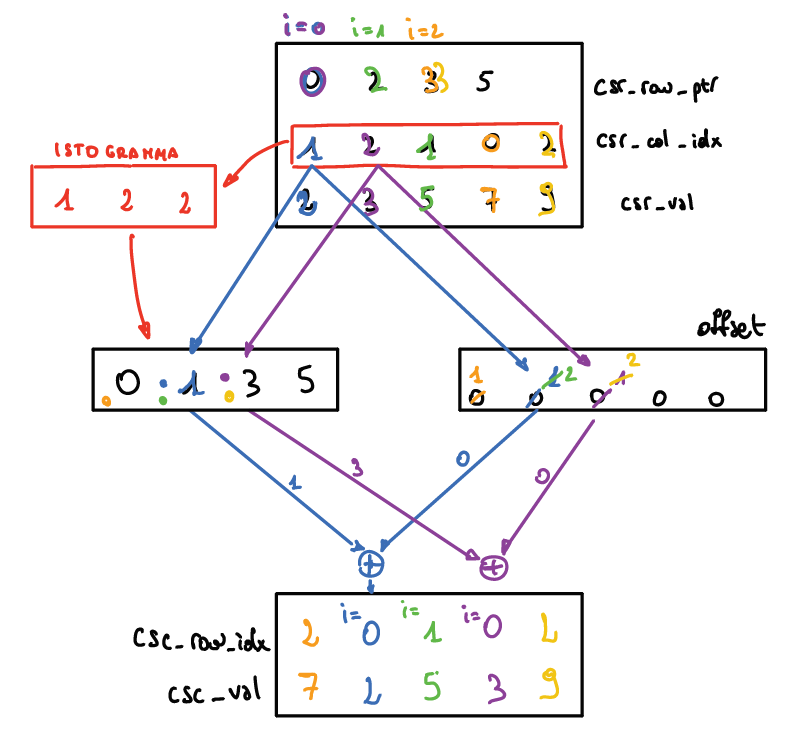
\includegraphics[scale=0.5]{transpose_algo_serial.PNG}
	\caption{Algoritmo seriale}
	\label{transpose_algo_serial}
\end{figure}

L'algoritmo si sviluppa nel seguente modo:
\begin{enumerate}
    \item si applica la funzione \emph{istogramma} \var{csr\_col\_idx} che calcola le occorrenze di ogni colonna, applicando \emph{scan} si ottiene il vettore \var{csc\_col\_ptr} (lunghezza $\mathrm{n}+1$) che conterrà i puntatori agli elementi di inizio riga trasposta;
    \item allochiamo il vettore \var{csc\_row\_idx} contente gli indici di riga (lunghezza $\mathrm{nnz}$);
    \item allochiamo il vettore \var{csc\_val} contente gli elementi non nulli (lunghezza $\mathrm{nnz}$);
    \item per ogni riga $i \in [0, m)$ processiamo gli elementi corrispondenti all'$i$-esima riga, legati alle posizioni $j \in [\var{csr\_row\_ptr}[i], \var{csr\_row\_ptr}[i+1])$
    \begin{itemize}
        \item la locazione $\mathrm{loc}$ del $j$-esimo elemento ordinata per righe è $\var{csc\_col\_ptr}[j] + \mathrm{offset}[j]$ dove $\mathrm{offset}[j]$ è un contatore incrementato ogni volta che aggiungiamo un elemento della colonna $\var{csc\_col\_ptr}[j]$;
        \item l'indice di riga dell'elemento $\mathrm{loc}$-esimo è $i$;
        \item il valore dell'elemento  $\mathrm{loc}$-esimo è $\var{csr\_val}[j]$.
    \end{itemize}
\end{enumerate}

L'esecuzione dell'algoritmo seriale è illustrato in Figura~\ref{transpose_algo_serial}.

\subsection{ScanTrans}

\begin{figure}[htbp]
    \centering
	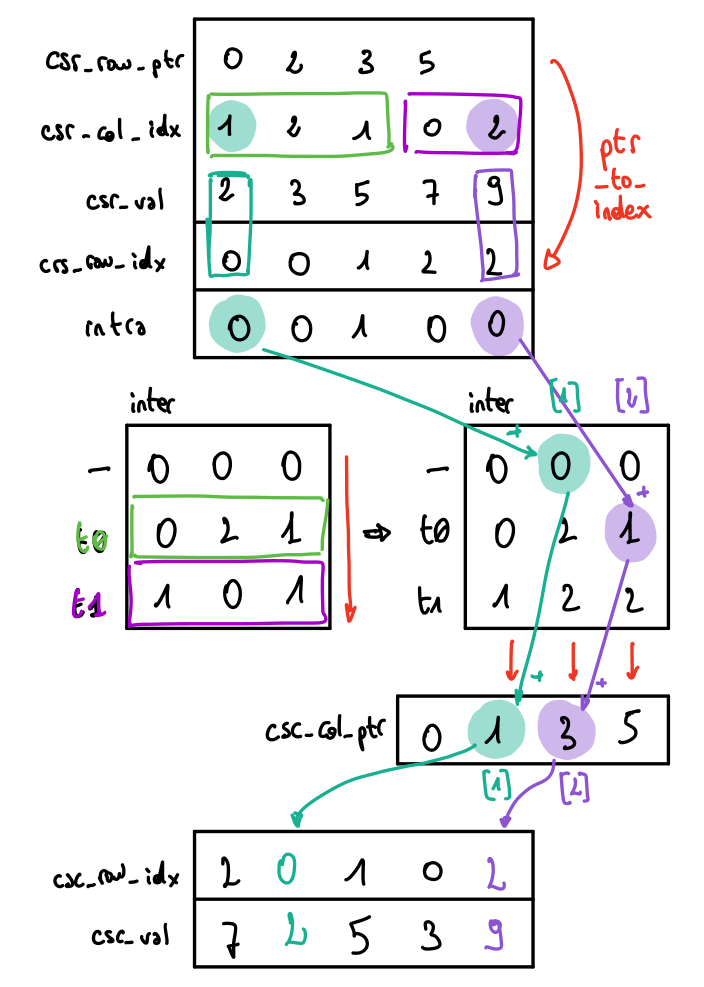
\includegraphics[scale=0.3]{transpose_scantrans.png}
	\caption{Algoritmo \ScanTrans}
	\label{transpose_algo_scantrans}
\end{figure}

L'algoritmo si sviluppa nel seguente modo:
\begin{enumerate}
    \item il vettore \var{csr\_row\_ptr} viene espanso per ottenere il vettore \var{csr\_row\_idx} attraverso la procedura \emph{pointers-to-indexes} che effettua l'operazione inversa dell'\emph{istogramma}; \\
    ora la struttura (\var{csr\_row\_idx}, \var{csr\_col\_idx}, \var{csr\_val}) rappresenta la matrice in formato COO ordinato per righe;
    \item decidiamo un numero arbitrario di thread $K$ che lavoreranno ciascuna su blocchi di $K/\mathrm{nnz}$ elementi. Allochiamo una matrice $\var{inter}$ di dimensioni $(K+1) \times n$ ed un vettore $\var{intra}$ di dimensione $\mathrm{nnz}$. La prima manterrà nella $(i+1)$-esima riga l'istogramma parziale relativo all'$i$-esimo blocco. La seconda mantiene un offset di colonna di ciascun elemento;
    \item i $K$ thread eseguono l'\emph{istogramma} ciascuna sul proprio blocco, la matrice $\var{inter}$ viene riempita;
    \item viene applicata l'operazione \emph{scan} ad ogni colonna della matrice \var{inter};
    \item il vettore \var{csc\_col\_ptr} viene ottenuto copiando l'ultima riga di \var{inter} ed applicando al vettore risultante l'operazione \emph{scan};
    \item riordiniamo gli elementi nei vettori \var{csr\_row\_idx}, \var{csr\_val} ottenendo quindi \var{csc\_row\_idx}, \var{csc\_val}; \\
    la nuova posizione dell'elemento $i$-esimo viene calcolata nel seguente modo:
    \begin{itemize}
        \item $b = i / \mathrm{nnz}$;
        \item $c = \var{csc\_col\_idx}[i]$;
        \item $l = \var{csc\_col\_ptr}[c] + \var{inter}[b n + c] + \var{inter}[c]$;
        \item $\var{csc\_val}[l] \leftarrow \var{csr\_val}[j]$;
        \item $\var{csc\_row\_idx}[l] \leftarrow \var{csr\_row\_idx}[j]$.
    \end{itemize}
\end{enumerate}

Il funzionamento dell'algoritmo è illustrato in Figura~\ref{transpose_algo_scantrans}. 

\subsection{MergeTrans}

\begin{figure}[htbp]
    \centering
	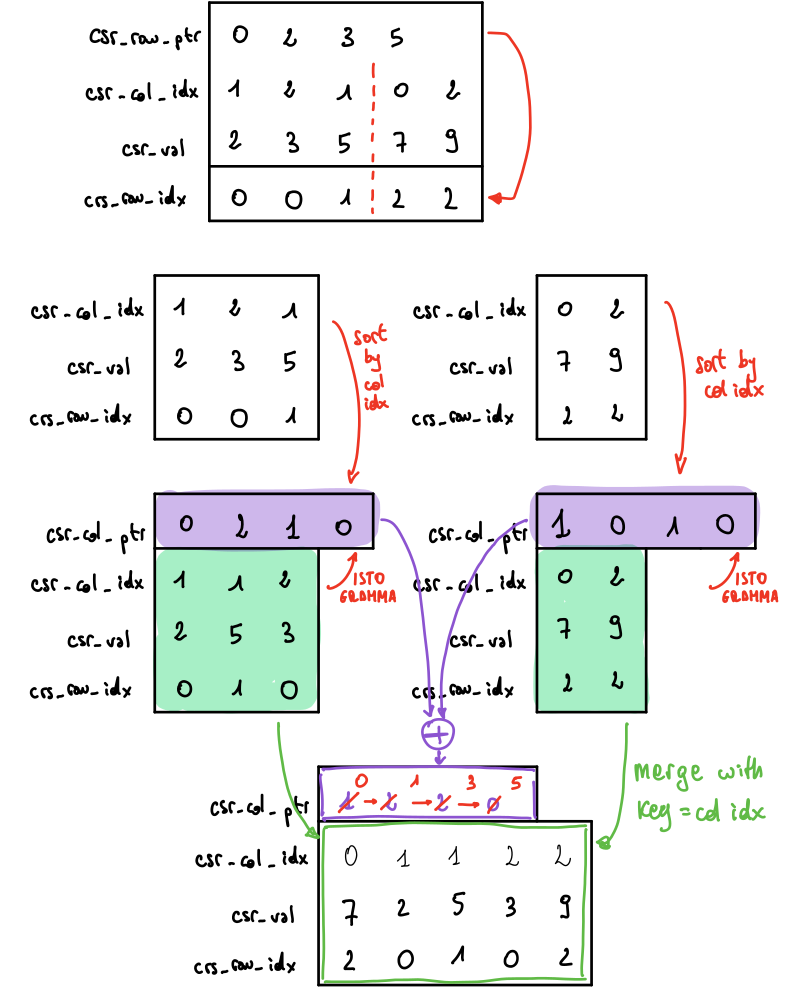
\includegraphics[scale=0.3]{transpose_mergetrans.png}
	\caption{Algoritmo \MergeTrans}
	\label{transpose_algo_mergerans}
\end{figure}
	
Il precedente algoritmo esegue nello step (6) un insieme di accessi casuali in memoria che non permettono di sfruttare in modo adeguato la shared memory. 

Per mitigare questo aspetto negativo viene introdotta una variante di questo algoritmo che, se implementato correttamente, permette ai thread di lavorare sempre con un numero costante, contiguo di elementi. 
	
L'algoritmo considerato prevede due passi importanti: \textit{sort} e \textit{merge}.
\begin{enumerate}
    \item portiamo la matrice in formato COO;
    \item i vettori viene segmentato in blocchi di dimensione omogenea ognuno dei quale viene ordinato per indice di colonna; ogni blocco mantiene il proprio array dei puntatori contenente l'istogramma parziale proprio del blocco;
    \item i blocchi vengono uniti a coppie attraverso l'operazione di \emph{merge} per ottenere blocchi di dimensione doppia della precedente. L'invariante di questo algoritmo è che ogni blocco mantiene la proprietà di essere ordinato per colonne ad ogni step.
\end{enumerate}

Questo algoritmo permette ad ogni griglia di thread di lavorare su una porzione di memoria ben definita, che eventualmente può essere caricata in più step nella shared memory a seconda di come viene implementato l'algoritmo che effettua il \emph{merge}. Il \emph{sort} viene applicato su blocchi di dimensione omogenea che deve essere scelta tale che l'intero blocco rientri nella shared memory.

Il funzionamento dell'algoritmo è illustrato in Figura~\ref{transpose_algo_mergerans}. 


\subsection{NVidia cuSPARSE}

I risultati temporali di tutti gli algoritmi precedentemente descritti saranno confrontati con l'implementazione di NVidia della trasposta della matrice sparsa. 

La libreria \cuSPARSE{} è parte di \textrm{CUDA Toolkit}, insieme di librerie utilizzate per effettuare operazioni tra vettori e matrici attraverso diversi formati. 

Versioni diverse di \textrm{CUDA Toolkit} implementano funzioni con nomi diversi e funzionamenti diversi. In particolare per \textrm{Cuda Toolkit 9.0} possiamo trasporre la matrice sparsa attraverso la procedura \texttt{cusparseScsr2csc}.

Nella versione \textrm{Cuda Toolkit 10.2} viene esposto il metodo \texttt{cusparseCsr2cscEx2} che effettua la trasposta in due possibili modi a seconda se il parametro ``algoritmo" è valorizzato con la costante \texttt{CUSPARSE\_CSR2CSC\_ALG1} oppure \texttt{CUSPARSE\_CSR2CSC\_ALG2}. Le due versioni differiscono per le tempistiche e per il consumo di memoria (maggior memoria necessaria per la seconda implementazione). Le tempistiche sono riportate in Tabella~\ref{results}.

La libreria è dettagliatamente documentata in \cite{cusparse}. A seconda della versione di \emph{CUDA} dobbiamo modificare lo script di compilazione. In particolare il \emph{Makefile} del progetto permette di compilare per due architetture specifiche, una con CUDA 9 e l'altra CUDA 10/11. 
	

\section{Procedure}\label{procedure}

I due algoritmi \ScanTrans e \MergeTrans vengono scomposti in diversi componenti, ognuno dei quali viene valutato nelle performance e testato separatamente. 

\subsection{Scan}
\label{scan}
Questa operazione prende in input un vettore $A = (a_0, a_1, ..., a_n)$ e ritorna un vettore $B=(I, a_0, a_0 \oplus a_1, ..., a_0 \oplus a_1 \cdots \oplus a_{n-1})$ con $\oplus$ è un'operazione binaria il cui elemento identità è $I$. Nel nostro caso l'operazione è la somma. 

L'algoritmo apparentemente sembra difficile da parallelizzare in quanto il risultato di ogni elemento dipende da tutti i gli elementi precedenti. Diverse soluzioni sono state proposte tra cui l'\emph{algoritmo di Blelloch}. Il suo funzionamento in due fasi è illustrato in Figura~\ref{scan_blelloch} e dettagliatamente discusso in \cite{scan}.

\begin{figure}[H]
	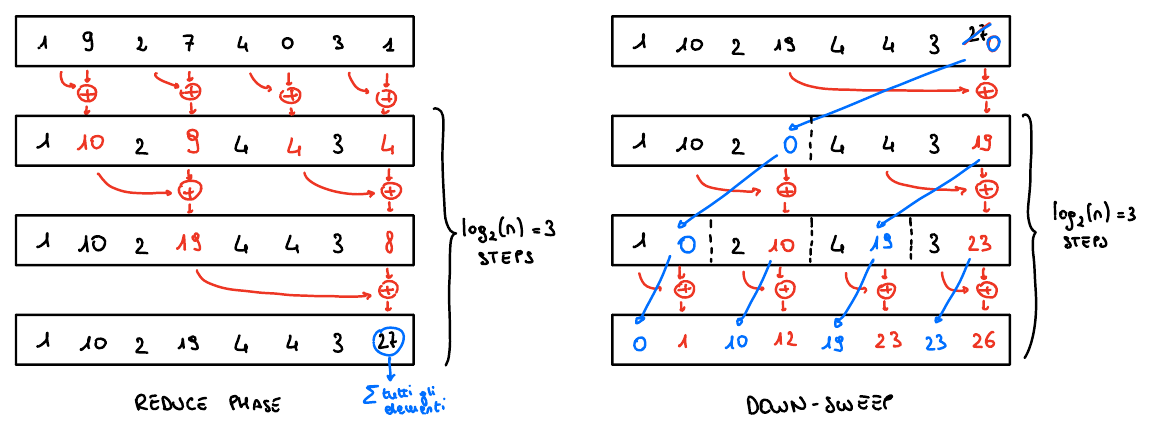
\includegraphics[scale=0.3]{scan.png}
	\caption{Algoritmo di Blelloch}
	\label{scan_blelloch}
\end{figure}

L'implementazione prevede che se l'intero vettore riesce ad essere memorizzato all'interno della shared memory di $N$ elementi, allora possiamo calcolare scan con una singola chiamata a kernel. 

Nel caso questo non sia possibile, l'operazione di scan viene segmentata, applicata separatamente a blocchi di $N$ elementi. Successivamente si mantiene un vettore di somme (vettore degli ultimi elementi del blocco), si applica ricorsivamente \emph{scan} su esso e si sommano gli offset ottenuti all'intero vettore di partenza. 

\subsection{Segmented sort}
\label{seg-sort}
Questa operazione prende in input un vettore di lunghezza $n$ ed un intero $\BlockSize$. Il vettore viene diviso in segmenti di lunghezza $\BlockSize$. Gli elementi di ogni segmento vengono permutati in modo che siano ordinati stabilmente. L'intero segmento deve rientrare nella shared memory.  

\begin{figure}[H]
\centering
	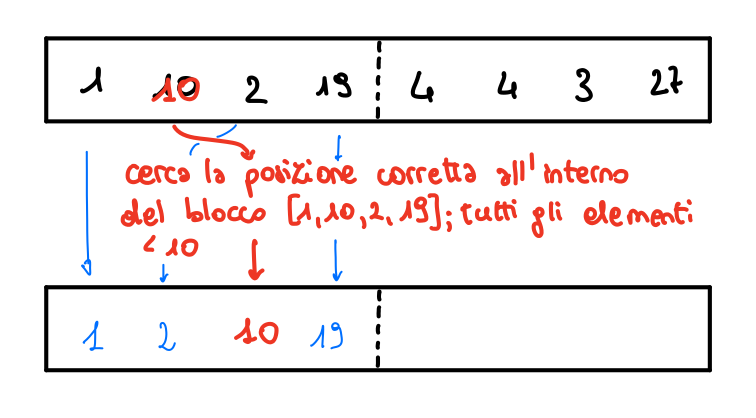
\includegraphics[scale=0.15]{segmented_sort.png}
	\caption{Segmented Sort}
	\label{segmented_sort}
\end{figure}

Una volta caricato il blocco in shared memory, la $i$-esima thread del blocco è incaricata di trovare la posizione corretta dell'$i$-esimo elemento all'interno del segmento, ed assegnarlo a tale posizione. L'algoritmo viene illustrato in Figura~\ref{segmented_sort}. 

L'ordinamento deve essere stabile quindi la posizione dell'$i$-esimo elemento di valore $y$ è dato dal numero di elementi $<y$, sommati al numero degli elementi $=y$ per indici $<i$. 

La dimensione ideale del blocco pari a $128$ elementi (caso interi a 32bit), ed è stata trovata empiricamente:
\begin{figure}[H]
	\centering
	\begin{tabular}{SS}
		\toprule
		\textbf{Thread per blocco} & \textbf{Performance (\si{\milli\second})} \\ \midrule
		128  & 2135.58 \\
		256  & 2139.62 \\
		512  & 2156.61  \\ \bottomrule
	\end{tabular}
	\caption{Performance su array di $2\cdot 10^7$ elementi}
\end{figure}

\subsection{Merge}
\label{merge}
L'operazione di \emph{merge} trasforma un vettore diviso in segmenti di dimensione $\BlockSize$ nel quale gli elementi di ogni segmento sono ordinati, in un vettore diviso in segmenti ordinati di dimensione $2 * \BlockSize$, ognuno dei quali è l'unione di una coppia di blocchi contigui. 

Differenziamo il caso in cui il blocco di dimensione $\BlockSize$ rientri o meno nella shared memory. 

\subsection{Merge small}

In questo caso una coppia di blocchi rientra completamente nella shared memory. In modo analogo a quanto fatto per l'operazione di \emph{segmented sort}, abbiamo un numero di thread per blocco pari a $\BlockSize$ nel quale l'$i$-esimo thread è incaricato di calcolare la posizione dell'$i$-esimo elemento. 

In questo caso la posizione dell'$i$-esimo elemento del blocco di sinistra è $i+j$ con $j$ posizione dell'elemento all'interno del blocco di destra, trovato attraverso una ricerca binaria in quanto i blocchi sono ordinati (differentemente da quanto avviene per il segmented sort). Analogamente lo stesso avviene per gli elementi del blocco di destra. 

A parità di valore, gli elementi del blocco di sinistra hanno indice minore di quelli di destra. 

\subsection{Merge big}

\begin{figure}[t]
    \centering
	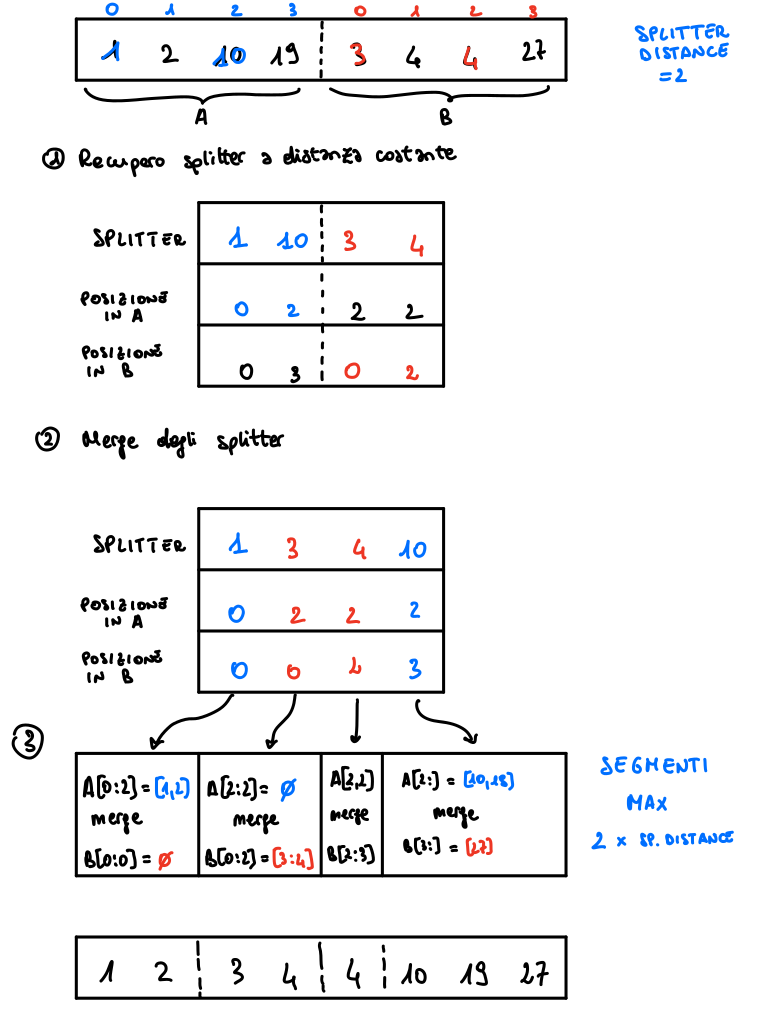
\includegraphics[scale=0.3]{merge_big.png}
	\caption{Merge big}
	\label{merge_big}
\end{figure}

Questo secondo algoritmo è illustrato in Figura~\ref{merge_big} ed originariamente preso da \cite{mergebig}. Applicando sempre \emph{merge small}, oltre che rinunciare alla shared memory, ogni thread del blocco dovrebbe lavorare su più di un elemento, aumentando la complessità della procedura. 

L'algoritmo proposto funziona nel seguente modo:
\begin{enumerate}
    \item recuperiamo dal vettore degli elementi segnaposto detti \emph{splitter} presi a distanza costante e pari ad $\SplitterDistance$; \\
    per ogni coppia di segmenti da unire ho una coppia di blocchi di splitter, trovo quindi la posizione di ogni splitter all'interno del blocco di destra ($A$) e di sinistra ($B$);
    \item applico \emph{merge} ricorsivamente sugli array di splitter;
    \item gli indici associati agli splitter dividono la coppia di blocchi in modo tale da poter effettuare tanti merge indipendenti da quanti sono gli splitter. \emph{Ogni merge indipendente considererà al massimo $2* \SplitterDistance$ elementi} (numero costante che scegliamo tale che rientri nella shared memory).
\end{enumerate}

La dimensione ideale del blocco pari a $256$ elementi (caso interi a 32bit), ed è stata trovata empiricamente:
\begin{figure}[H]
	\centering
	\begin{tabular}{SS}
		\toprule
		\textbf{Thread per blocco} & \textbf{Performance (\si{\milli\second})} \\ \midrule
		128  & 708.87  \\	
		256  & 701.54 \\
		512  & 715.71 \\ \bottomrule
	\end{tabular}
	\caption{Performance su array di $2\cdot 10^7$ elementi}
\end{figure}
Mentre il valore migliore per la distanza degli splitter (\SplitterDistance) è di $ 128 $.

\subsection{Istogramma / Index to pointers}
\label{idx-to-pnt}
Dato un vettore $A$ di $n$ elementi compresi tra $0$ ed $m-1$ riceviamo un vettore di $m$ elementi nel quale l'$i$-esima cella contiene la frequenza con cui il valore $i$ è presente in $A$. 

L'algoritmo si sviluppa in due fasi:
\begin{enumerate}
    \item il vettore $A$ viene diviso in $N$ segmenti di lunghezza omogenea, ogni segmento viene processato da un blocco di thread che mantiene l'istogramma parziale;
    \item gli istogrammi parziali vengono poi uniti attraverso un'operazione di prefix scan che si effettua ``in verticale''. Tale operazione può essere ottenuta:
    \begin{itemize}
        \item trasponendo la matrice degli istogrammi parziali ed applicando $N$ volte \emph{prefix sum}; oppure
        \item attraverso $N$ blocchi di thread che attraversano sequenzialmente il vettore colonna degli istogrammi parziali.
    \end{itemize}
    \item si applica \emph{prefix sum} sul risultato dell'operazione precedente.
\end{enumerate}

L'algoritmo è illustrato in Figura~\ref{index_to_pointers}. 

\begin{figure}[t]
    \centering
	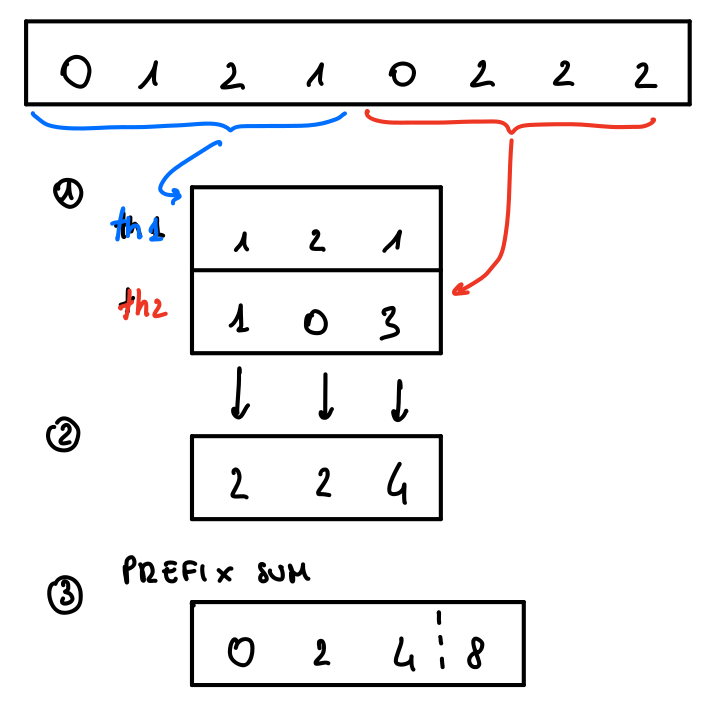
\includegraphics[scale=0.22]{index_to_pointers.png}
	\caption{Index to pointers}
	\label{index_to_pointers}
\end{figure}


La dimensione ideale del blocco pari a $32$ elementi (caso interi a 32bit), ed è stata trovata empiricamente:
\begin{figure}[H]
	\centering
	\begin{tabular}{SS}
		\toprule
		\textbf{Thread per blocco} & \textbf{Performance (\si{\milli\second})} \\ \midrule
		1 & 1016.87 \\
		32 & 1013.65 \\
		64 & 1024.70 \\
		256 & 986.84 \\ \bottomrule
	\end{tabular}
	\caption{Performance su array di $10^6$ elementi} % da 999'999 a 1'000'000
\end{figure}

\subsection{Pointers to index}
\label{pnt-to-idx}
Operazione inversa di \emph{index to pointers}. Il vettore risultante è ordinato. Può essere implementato assegnando ad ogni blocco di thread un elemento del vettore delle frequenze da espandere. 

L'algoritmo è illustrato in Figura~\ref{pointers_to_index}. 

\begin{figure}[t]
    \centering
	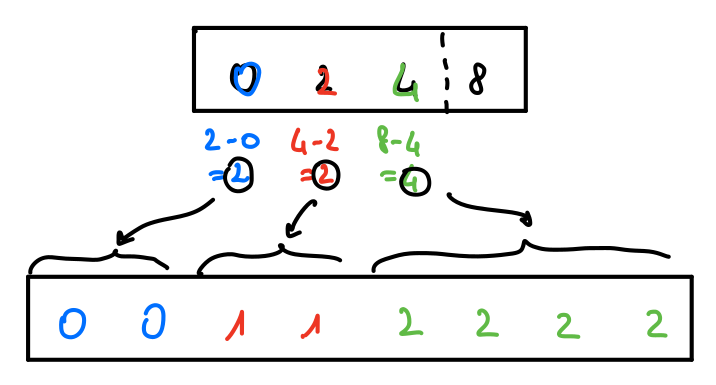
\includegraphics[scale=0.22]{pointers_to_index.png}
	\caption{Pointers to index}
	\label{pointers_to_index}
\end{figure}

La dimensione ideale del blocco pari a $32$ elementi (caso interi a 32bit), ed è stata trovata empiricamente:
\begin{figure}[H]
	\centering
	\begin{tabular}{SS}
		\toprule
		\textbf{Thread per blocco} & \textbf{Performance (\si{\milli\second})} \\ \midrule
		1 & 2328.88 \\
		16 & 2375.74 \\
		32 & 2322.75 \\
		1024 & 3326.13 \\ \bottomrule
	\end{tabular}
	\caption{Performance su array di $2\cdot 10^7$ elementi} 
\end{figure}



\section{Struttura dell'implementazione}\label{struttura}

L'intera implementazione è scaricabile attraverso \emph{git} dalla repository \url{https://github.com/michelepenzo/architetture-avanzate}.

La struttura delle directory del progetto è presente in Figura~\ref{fig:struct}. 

La sottodirectory \emph{doc} contiene questo stesso documento in formato \emph{pdf} ed i rispettivi sorgenti \emph{tex}. 

La sottodirectory \emph{code} contiene i sorgenti dell'applicativo principale e di quello secondario di test. 

Lo scopo del primo è generare un file \emph{csv} contente le tempistiche e gli speedup di ogni algoritmo applicato sulle istanze di matrici in input generate casualmente oppure lette da file \emph{mtx} (\emph{market matrix}, una rappresentazione della matrice sparsa in formato COO attraverso file di testo). 

Lo scopo del secondo applicativo è testare il corretto funzionamento di ogni componente del progetto. In particolare, vengono sottoposte le stesse istanze di array o matrici (a seconda del componente che sta per essere testato) sia alla funzione che ne implementa l'algoritmo parallelo, sia alla funzione che ne implementa l'algoritmo seriale. Ovviamente ci si aspetta che i risultati siano uguali per tutte le istanze.

\begin{figure}
    \dirtree{%
	.1 root.		
	    .2 README.md.
		.2 doc.			
		.2 code.
			.3 {matrices}.
			.3 {include}.
				.4 {matrix.hh}.
				.4 {merge\_step.hh}.
				.4 {procedures.hh}.
				.4 {transposers.hh}.
				.4 {Timer.$ * $}.
				.4 {utilities.hh}.
			.3 {src}.
				.4 {...}.
				.4 {transposer.cu}.
				.4 {main.cu}.
			.3 {test}.	
				.4 {...}.
				.4 {tester.hh}.
				.4 {test\_main.cu}.
			.3 Makefile.			
			.3 {timing\_analysis.csv}.	
}
    \caption{Struttura delle directory del progetto}
    \label{fig:struct}
\end{figure}

In particolare:
\begin{itemize}
    \item il file \texttt{include/matrix.hh} contiene le classi \emph{FullMatrix} e \emph{SparseMatrix} che si occupano di allocare nella memoria host lo spazio necessario a contenere la matrice date le sue specifiche ($m$, $n$, $nnz$), sia come matrice estesa sia in formato \emph{csr}. Inoltre contiene i metodi per inizializzare la matrice in modo casuale e per passare da un formato all'altro;
    \item il file \texttt{include/utils.hh} contiene i metodi di utilità quali le funzioni di stampa e di allocazione e deallocazione della memoria device;
    \item i file \texttt{include/procedures.hh} e \texttt{merge\_step.hh} contengono le dichiarazioni delle procedure descritte nella Sezione~\ref{procedure}. La maggior parte delle definizioni sono presenti nella sottodirectory \texttt{src}, nel caso del metodo \emph{merge\_step} la definizione è scritta direttamente nell'header. Questa scelta è conveniente in quanto tale funzione è definita rispetto ad un tipo generico, se la definizione fosse stata riportata nei file cpp avremmo dovuto indicare esplicitamente i tipi concreti per il quale vogliamo rendere disponibile il nostro metodo (\cite{template});
    \item il file \texttt{include/transposers.hh} e rispettivo sorgente \texttt{src/transposers.cu} contengono le dichiarazioni e definizioni dei metodi che effettuano la trasposta: seriale, parallela con \ScanTrans{} e \MergeTrans{} ed infine da libreria \cuSPARSE{} con entrambi i possibili algoritmi;
    \item i file \texttt{Timer.*} contengono una classe di utilità \emph{timer} che permette di cronometrare il tempo che occorre per eseguire un dato pezzo di codice;
    \item il file \texttt{src/main.cu} contiene l'applicativo principale che chiama i diversi metodi di trasposta sulla matrice fornita in input, ne cronometra le tempistiche e le stampa in output;
    \item il file \texttt{test/tester.hh} contiene la classe astratta \emph{tester} che espone un metodo \emph{test\_many\_instances} che chiama un metodo astratto \emph{test} un numero arbitrario di volte, passandogli in input un intero che rappresenta il numero dell'istanza attuale che può essere usato per decidere la dimensione dell'istanza di test. Attualmente le istanze testate vanno da 1 a 20'000, poi da 20'000 a 20'000'000 con step $\times 1.5$; 
    \item i file \texttt{test/tester\_*.hh} si occupano di testare un singolo componente, contengono ciascuna uno o più classi concrete che estendono la classe astratta \emph{tester};
    \item il file \texttt{test/test\_main.cu} contiene l'applicativo di test che alloca oggetti delle varie classi tester, li avvia e ne stampa gli eventuali errori a video.
\end{itemize}
	
\section{Avvio degli applicativi}

L'applicativo principale può essere avviato con tre modalità diverse:
\begin{itemize}
    \item senza parametri, genera una matrice $500'000\times 500'000$ con $10'000'000$ elementi non nulli, ne valuta le tempistiche con i diversi algoritmi ritornando la media su un numero arbitrario di esecuzioni;
    \item con tre parametri interi $\mathrm{m}$, $\mathrm{n}$, $\mathrm{nnz}$, genera una matrice avente le dimensioni ricevute in input e procede alla valutazione delle tempistiche come sopra;
    \item con un parametro stringa \texttt{filename}, legge da file una matrice che deve essere nel formato \emph{mtx market matrix}.
\end{itemize}

Avviando l'applicativo principale attraverso il Makefile con \emph{make run} viene avviato molteplici volte l'applicativo principale, ogni volta con un'istanza di matrice diversa in input, con lo scopo di popolare un documento \emph{timing\_analysis.csv} contenente le tempistiche medie su diversi input. 

L'applicativo di test di avvia con una sola modalità equivalentemente avviando il nome dell'applicativo senza parametro oppure attraverso il Makefile con \emph{make test}. Su \emph{stdout} viene stampato ``no" se almeno un test ha mostrato anomalie, ``ok" altrimenti. 

\begin{figure*}[t]
    \centering
    \scalebox{0.9}{
    \begin{tabular}{lS[table-format=7.0] S[table-format=7.0] S[table-format=8.0] S[table-format=4.2] S[table-format=4.2] S[table-format=4.2] S[table-format=4.2] S[table-format=4.2]}
    \toprule
    \textbf{Nome} 
    & \textbf{M}
    & \textbf{N}
    & \textbf{NNZ}
    & \textbf{Serial}
    & \textbf{\ScanTrans{}}
    & \textbf{\MergeTrans{}}
    & \textbf{\cuSPARSE{} 1}
    & \textbf{\cuSPARSE{} 2}
    \\ \midrule
    language.mtx	
        & 399130
        & 399130
        & 1216334
        &  55.75
        & 114.71
        & 197.05
        & 122.02
        &  18.36 \\
    webbase-1M.mtx	
        & 1000005	
        & 1000005
        & 3105536	
        & 138,84	
        & 278,55	
        & 520,90
        & 149,81	
        &  51,00 \\
    rajat21.mtx	
        & 411676	
        & 411676	
        & 1893370	
        &  77,97	
        & 147,64	
        & 306,56	
        & 127,31	
        &  26,77 \\
    ASIC\_680k.mtx	
        & 682862	
        & 682862	
        & 3871773	
        & 154,37	
        & 265,47	
        & 844,76	
        & 155,31	
        &  56,74 \\
    memchip.mtx	
        & 2707524	
        & 2707524	
        & 14810202	
        &  594,18	
        &  994,62	
        & 2328,67	
        &  298,93	
        &  188,07 \\
    cant.mtx	
        & 62451	
        & 62451	
        & 2034917	
        &  73,83	
        & 114,40	
        & 248,49	
        & 127,26	
        &  31,11 \\
    FullChip.mtx	
        & 2987012	
        & 2987012	
        & 26621990	
        &  997,37	
        & 1543,02	
        & 9481,42	
        &  454,53	
        &  328,32 \\
    stomach.mtx	
        & 213360	
        & 213360	
        & 3021648	
        & 110,84	
        & 164,30
        & 387,78	
        & 139,57	
        &  40,26 \\
    web-Google.mtx	
        & 916428	
        & 916428	
        & 5105039	
        &  399,63	
        &  382,37	
        & 3327,56	
        &  170,59	
        &   73,25 \\
    random	
        & 100000	
        & 100000	
        & 10000000	
        &  898,99	
        &  475,17	
        & 3056,12	
        &  210,57	
        &  130,25 \\
    random	
        & 100000	
        & 100000	
        & 10000000	
        &  902,23	
        &  475,72	
        & 3060,25	
        &  208,22	
        &  133,22 \\
    random	
        & 150000	
        & 200000	
        & 5000000	
        &  523,66	
        &  263,90	
        & 1351,83	
        &  161,90	
        &   72,70 \\
    random	
        & 150000	
        & 200000	
        & 5000000	
        &  527,15	
        &  262,88	
        & 1353,93	
        &  165,19	
        &   74,98 \\
    random	
        & 500000	
        & 500000	
        & 10000000	
        & 1380,96	
        &  532,76	
        & 2853,55	
        &  227,33	
        &  141,18 \\ \bottomrule
    \end{tabular}}
    \caption{Risultati sperimentali -  $\textrm{M}, \textrm{N}, \textrm{NNZ}$ rispettivamente numero di righe, di colonne, di elementi non nulli della matrice. I tempi sono in \si{\milli\second}.}
    \label{results}
\end{figure*}

\begin{figure*}[t]
    \centering
    \scalebox{0.9}{
    \begin{tabular}{lS[table-format=7.0] S[table-format=7.0] S[table-format=8.0] S[table-format=4.2] S[table-format=4.2] S[table-format=4.2] S[table-format=4.2] S[table-format=4.2]}
    \toprule
    \textbf{Nome} 
    & \textbf{M}
    & \textbf{N}
    & \textbf{NNZ}
    & \textbf{Serial}
    & \textbf{\ScanTrans{}}
    & \textbf{\MergeTrans{}}
    & \textbf{\cuSPARSE{} 1}
    & \textbf{\cuSPARSE{} 2}
    \\ \midrule
    language.mtx	
        & 399130	
        & 399130	
        & 1216334	
        & 1.00
        & 0.49	
        & 0.28	
        & 0.46	
        & 3.04 \\
    webbase-1M.mtx	
        & 1000005	
        & 1000005	
        & 3105536	
        & 1.00
        & 0.50	
        & 0.27	
        & 0.93	
        & 2.72 \\
    rajat21.mtx	
        & 411676	
        & 411676	
        & 1893370	
        & 1.00
        & 0.53	
        & 0.25	
        & 0.61	
        & 2.91 \\
    ASIC\_680k.mtx	
        & 682862	
        & 682862	
        & 3871773	
        & 1.00
        & 0.58	
        & 0.18	
        & 0.99	
        & 2.72 \\
    memchip.mtx	
        & 2707524	
        & 2707524	
        & 14810202	
        & 1.00
        & 0.60	
        & 0.26	
        & 1.99	
        & 3.16 \\
    cant.mtx	
        & 62451	
        & 62451	
        & 2034917	
        & 1.00
        & 0.65	
        & 0.30	
        & 0.58	
        & 2.37 \\
    FullChip.mtx	
        & 2987012	
        & 2987012	
        & 26621990	
        & 1.00
        & 0.65	
        & 0.11	
        & 2.19	
        & 3.04 \\
    stomach.mtx	
        & 213360	
        & 213360	
        & 3021648	
        & 1.00	
        & 0.67	
        & 0.29	
        & 0.79	
        & 2.75 \\
    web-Google.mtx	
        & 916428	
        & 916428	
        & 5105039	
        & 1.00
        & 1.05	
        & 0.12	
        & 2.34	
        & 5.46 \\
    random	
        & 100000	
        & 100000	
        & 10000000	
        & 1.00	
        & 1.89	
        & 0.29	
        & 4.27	
        & 6.90 \\
    random	
        & 100000	
        & 100000	
        & 10000000	
        & 1.00	
        & 1.90	
        & 0.29	
        & 4.33	
        & 6.77 \\
    random
        & 150000	
        & 200000	
        & 5000000	
        & 1.00	
        & 1.98	
        & 0.39	
        & 3.23	
        & 7.20 \\
    random
        & 150000	
        & 200000	
        & 5000000	
        & 1.00	
        & 2.01	
        & 0.39	
        & 3.19	
        & 7.03 \\
    random
        & 500000	
        & 500000	
        & 10000000	
        & 1.00	
        & 2.59	
        & 0.48	
        & 6.07	
        & 9.78 \\ \bottomrule
    \end{tabular}}
    \caption{Risultati sperimentali -  Speedup}
    \label{results_speedup}
\end{figure*}







\section{Risultati sperimentali}

Confrontiamo ora le performance delle varie implementazioni che seguono:
\begin{itemize}
    \item seriale;
    \item parallela \emph{scan trans};
    \item parallela \emph{merge trans};
    \item \cuSPARSE (entrambi gli algoritmi).
\end{itemize}

Le istanze su cui vengono eseguiti i vari algoritmi sono in parte generate in modo casuale (a partire dalle specifiche della matrice sparsa), in parte recuperate dal dataset "University  of Florida sparse  matrix collection`` \cite{dataset}. Tale dataset è stato usato per valutare le performance degli algoritmi in \cite{parallelTrans}.

La macchina sul quale vengono eseguiti i vari algoritmi è equipaggiata con una scheda NVidia GeForce GTX 780 con Cuda Runtime 10.2.

I risultati sono visibili in Tabella~\ref{results}. 

\section{Considerazioni finali}\label{conclusioni}
	% tirare le somme di cosa abbiamo ottenuto
	% cosa migliorare?
	% come possiamo continuare il progetto se avessimo avuto più tempo?
		% algo merge con merge buffer che è gia implementato
		% testare l'efficienza delle componenti rispetto alla implementazione nvidia
		% idx to pntrs (soffre race condition) --> un thread ha un blocco
		
\bibliographystyle{IEEEtran}
\bibliography{biblio}
\newpage
\mbox{}
\end{document}
